\chapter{\IfLanguageName{dutch}{Stand van zaken}{State of the art}}
\label{ch:stand-van-zaken}

% Tip: Begin elk hoofdstuk met een paragraaf inleiding die beschrijft hoe
% dit hoofdstuk past binnen het geheel van de bachelorproef. Geef in het
% bijzonder aan wat de link is met het vorige en volgende hoofdstuk.

% Pas na deze inleidende paragraaf komt de eerste sectiehoofding.

Om de verschillende 'ontgoogle' methoden met elkaar te kunnen vergelijken, moeten we eerst wat dieper ingaan op de verschillende Google componenten die te vinden zijn binnen het Android besturingssysteem en hoe deze zoveel mogelijk te limiteren en/of uit te schakelen zijn. Dit hoofdstuk zal toelichten wat er precies gebeurt achter de schermen van Android en hoe precies een 'ontgoogling' kan gebeuren. Bijkomend wordt ook het Huawei handelsverbod besproken en wat het raakpunt daarvan is met dit werk.

\section{Google componenten binnen Android}
Google software binnen het Android besturingssysteem wordt beschreven als de overkoepelende term 'Google Apps'. Deze kan verder opgedeeld worden in de 'Google Play Services', het achterliggende 'brein' van Google, en Google applicaties, zoals GMail, Google Play Store, etc.

\subsection{Google Play Services}
Vlakbij het hart van het Android besturingssysteem liggen de 'Google Play Services'. Deze services zijn zeer nauw geïntegreerd in het Android besturingssysteem, en bieden een bundel van API's aan \autocite{marshall_google-play-services}. Een API of 'Application Program Interface' is kort gezegd een set van hulpmiddelen die het voor applicatie-ontwikkelaars makkelijker maakt om applicaties te ontwikkelen \autocite{beal_api}.

AOSP, ook gekend als Android Open Source Project, is de basis van het Android besturingssysteem. Zoals de naam zelf al zegt, is dit project volledig 'open-source'. Dit houdt in dat iedereen vrij is om de broncode te gebruiken en aan te passen. 

De Android versie die op de smartphone van de meeste mensen is geïnstalleerd, is echter niet volledig 'open-source' maar ook voor een deeltje 'closed-source'. Smartphone producenten voeren vaak zelf nog wijzigingen door op AOSP, die de gebruikerservaring aanpassen. Zo kunnen hun wijzigingen invloed hebben op het visuele aspect van het besturingssysteem, extra functionaliteiten toevoegen en er voor zorgen dat alle hardware die gebruikt wordt binnen het apparaat ook ondersteund wordt door apparaat-specifieke drivers. Ook worden er vaak extra applicaties meegeleverd, die al dan niet geïnstalleerd zijn als een systeemapplicatie. Applicaties die standaard worden meegeleverd met het apparaat, maar door gebruikers als onnodig bestempeld worden, worden 'bloatware' genoemd. Op deze manier ontwikkelt Xiaomi voor haar apparaten een eigen versie van Android die ze MIUI noemen, OnePlus ontwikkelt een eigen versie van Android die ze OxygenOS noemen, LG heeft LG UX, etc. Voor de westerse markt worden de Google Apps vaak opgenomen in het besturingssysteem. Google zelf biedt ook Android telefoons aan, zoals de reeds verouderde 'Nexus' apparaatlijn en de huidige 'Pixel' apparaatlijn. Zelfs het besturingssysteem dat op deze apparaten draait is een aangepaste versie van het AOSP, ook al worden hun apparaten vaak als de apparaten met de 'schoonste' versie van Android beschouwd. Binnen hun versie van Android is ook het closed-source software paket 'Google Apps' aanwezig \autocite{torres_stockandroid}. Steeds meer producenten bieden apparaten aan met een zo min mogelijk aangepaste versie van Android, om zo beroep te doen op mensen die op zoek zijn naar de 'stock experience'. Doordat er minder extra functionaliteiten moeten geïmplementeerd worden, zorgt dit voor de fabrikant ook dat er minder tijd en werk moet worden gestoken in de ontwikkeling. Ook de update cyclus kan zo sneller verlopen, wat vaak een knelpunt is bij apparaten die op een aangepaste versie van Android draaien \autocite{manik_slow-updates}. 

Een fenomeen dat voortkomt uit trage update cycli, is Android fragmentatie. Dit fenomeen houdt in dat een groot deel van de Android apparaten niet de mogelijkheid heeft om op de laatste versie van Android te draaien. Zo kan er geen gebruik gemaakt worden van de nieuwste functies, maar wat nog belangrijker is, is dat gebruikers niet beschikken over de nieuwste veiligheidsupdates, wat een zeer groot risico inhoudt. Op het 'Distribution dashboard' van Android, te zien op figuur \ref{fig:androidfragmentation}, wordt ook aangetoond dat op 7 mei 2019 nog maar 10,4\% van Android apparaten beschikt over de laatste versie van het besturingssysteem, namelijk Android Pie (9.0), die officiëel werd vrijgegeven op 6 augustus 2018.

\begin{figure}
    \centering
    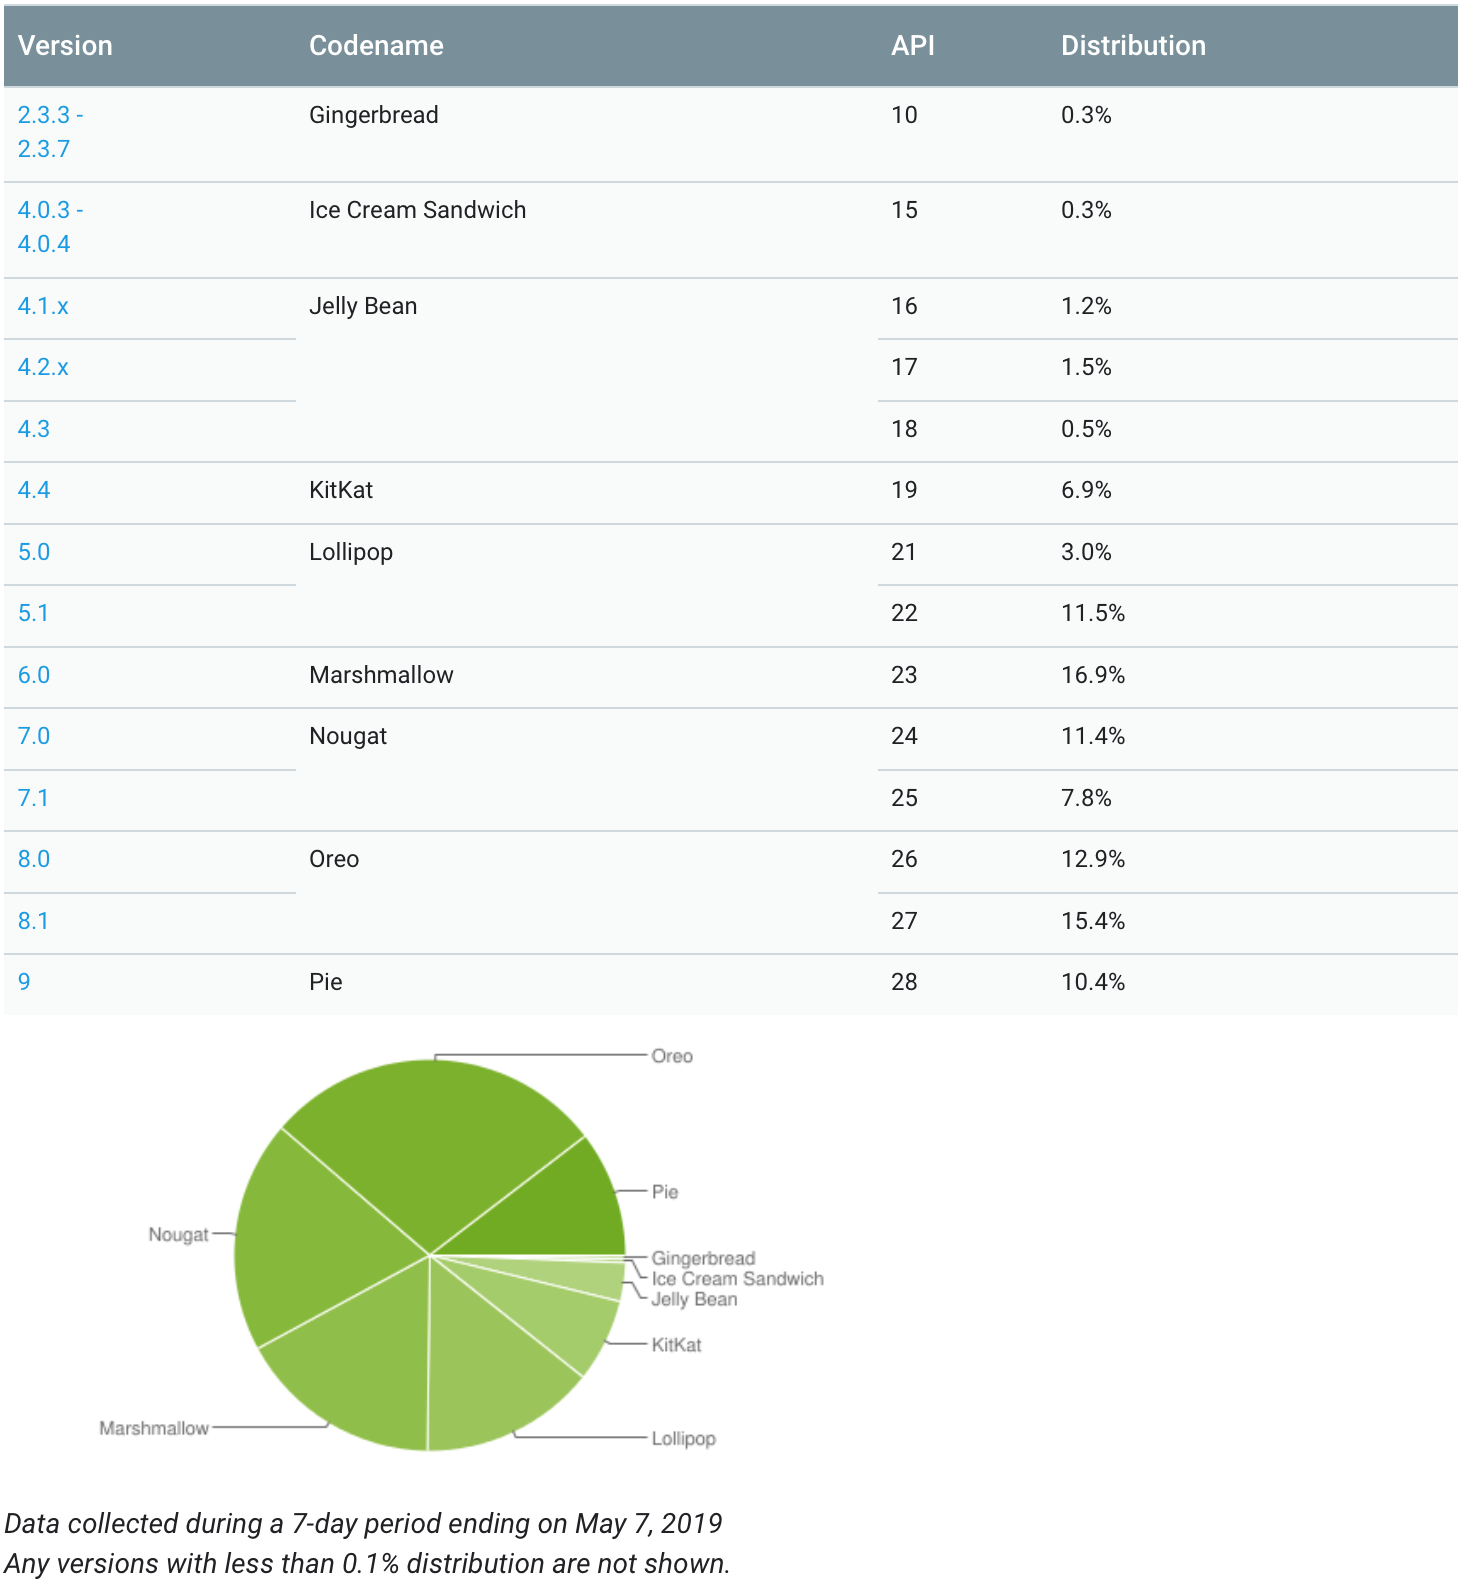
\includegraphics[width=0.8\textwidth]{img/fragmentation.png}
    \caption{Distributie van Android versies op 7 mei 2019}
    \label{fig:androidfragmentation}
    \medskip
    \small
    https://developer.android.com/about/dashboards
\end{figure}

Via het 'Android One' programma dat Android aanbiedt, is het makkelijker voor producenten om een 'stock experience' aan te bieden. Hierbij wordt een technische standaard vastgelegd waaraan de apparaten moeten voldoen. Het doel van dit programma is om een consistente gebruikerservaring aan te bieden en te zorgen dat software-updates veel makkelijker te voorzien zijn, aangezien deze rol verlegd wordt naar Google in plaats van de fabrikant zelf. Ook in deze versie van Android zijn Google Apps inbegrepen \autocite{android_androidone}.  Dit deel omvat dan alle applicaties van Google zelf, bv. GMail, Google Maps, en de onderliggende 'Google Play Services' \autocite{amadeo_open-source}.

AOSP biedt een bundel API's  aan, maar Google zelf adviseert om de API's van de Google Play Services te gebruiken. Deze zijn immers een stuk makkelijker te gebruiken, en zorgen ervoor dat applicaties niet rechtstreeks afhankelijk zijn van Android besturingssysteem updates. Dit komt doordat de Play Services applicatie apart van het besturingssysteem wordt bijgewerkt. Applicatie ontwikkelaars kunnen dan ook gebruikmaken van de nieuwste functie's binnen deze API's. Zo moeten ze veel minder terugvallen op gedateerde API's om zo hun applicatie compatibel te maken met oudere versies van Android.  Deze API's van de Play Services zijn dan ook 'closed-source', tegenover de API's van AOSP, die 'open-source' zijn \autocite{marshall_google-play-services}. 

Een voorbeeld hiervan is de locatie service. AOSP biedt een 'Location API' aan. Wanneer een applicatie gebruik maakt van deze API, moet er expliciet gekozen worden tussen 3 'location providers'. Elk van deze gebruikt een verschillende manier om de locatie van een gebruiker te bepalen \autocite{android_location-strategies}. De GPS provider gebruikt de fysieke GPS chip binnen het apparaat, en kan hierdoor ook de meest accurate locatiegegevens teruggeven, maar deze verbruikt ook het meeste energie. De netwerk provider maakt gebruik van de GPS chip, samen met gegevens van het mobiele netwerk om zo een snelle initiële verbinding te krijgen. De nauwkeurigheid van de locatiegegevens die hier worden teruggeven is lager, maar deze methode zorgt wel voor een lager energieverbruik. Tenslotte is er ook de passieve provider. Deze zal, in tegenstelling tot de andere providers, niet actief zoeken naar een verbinding. In plaats daarvan, maakt deze gebruik van locatiegegevens die verschaft werden door de andere providers, wanneer deze door andere applicaties worden aangesproken \autocite{idris_location-providers}. De Google Play Services Location API heeft als voordeel dat ontwikkelaars niet expliciet meer moeten kiezen tussen één van deze drie providers. Deze keuze wordt automatisch gemaakt zodat nauwkeurigheid en energieverbruik geoptimaliseerd wordt \autocite{android_location-strategies}.

\blockcquote{android_location-strategies}{
    The Google Location Services API, part of Google Play Services, provides a more powerful, high-level framework that automatically handles location providers, user movement, and location accuracy. It also handles location update scheduling based on power consumption parameters you provide. In most cases, you'll get better battery performance, as well as more appropriate accuracy, by using the Location Services API.
}

Steeds meer en meer open-source applicaties, die voorheen te vinden waren binnen AOSP, worden achtergelaten in hun ontwikkeling en vervangen door een closed-source versie op de Google Play Store, de applicatie van Google waarmee gebruikers applicaties kunnen downloaden en installeren. AOSP applicaties die niet meer verder ontwikkeld worden, zijn vaak niet meer zo robuust als Google's vervangende applicatie, en zien er ook gedateerd uit. Enkele voorbeelden van achtergelaten AOSP applicaties en hun vervangende product van Google, zijn te zien in figuren \ref{fig:googlesearch}, \ref{fig:googleplaymusic} en \ref{fig:googlecalendar}. Deze vervangende applicaties kunnen ook automatisch bijgewerkt worden, tegenover de AOSP applicaties die een systeemupdate vereisen om bijgewerkt te worden. Ook de Play Store maakt gebruik van de Google Play Services om applicaties automatisch te kunnen updaten. Op deze manier probeert Google haar eigen applicaties zoveel mogelijk macht te geven tegenover de 'open-source' applicaties binnen AOSP \autocite{amadeo_open-source}.

\begin{figure}
    \centering
    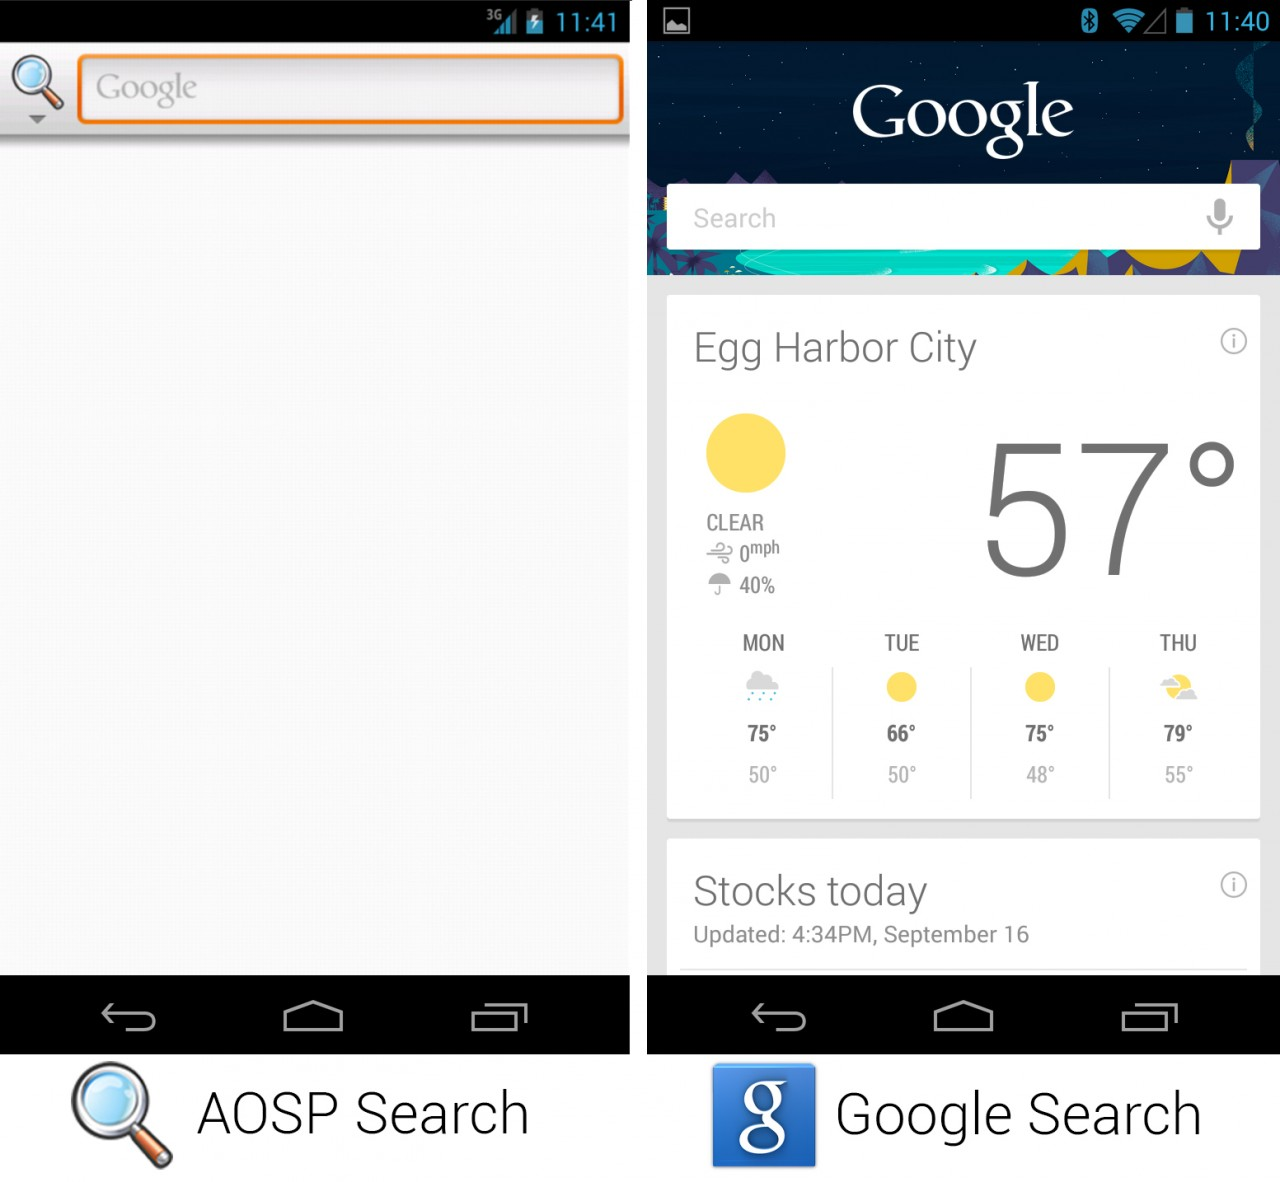
\includegraphics[width=0.55\textwidth]{img/googlesearch.jpg}
    \caption{AOSP zoekapplicatie vergeleken met Google's zoekapplicatie}
    \label{fig:googlesearch}
    \autocite{amadeo_open-source}
\end{figure}

\begin{figure}
    \centering
    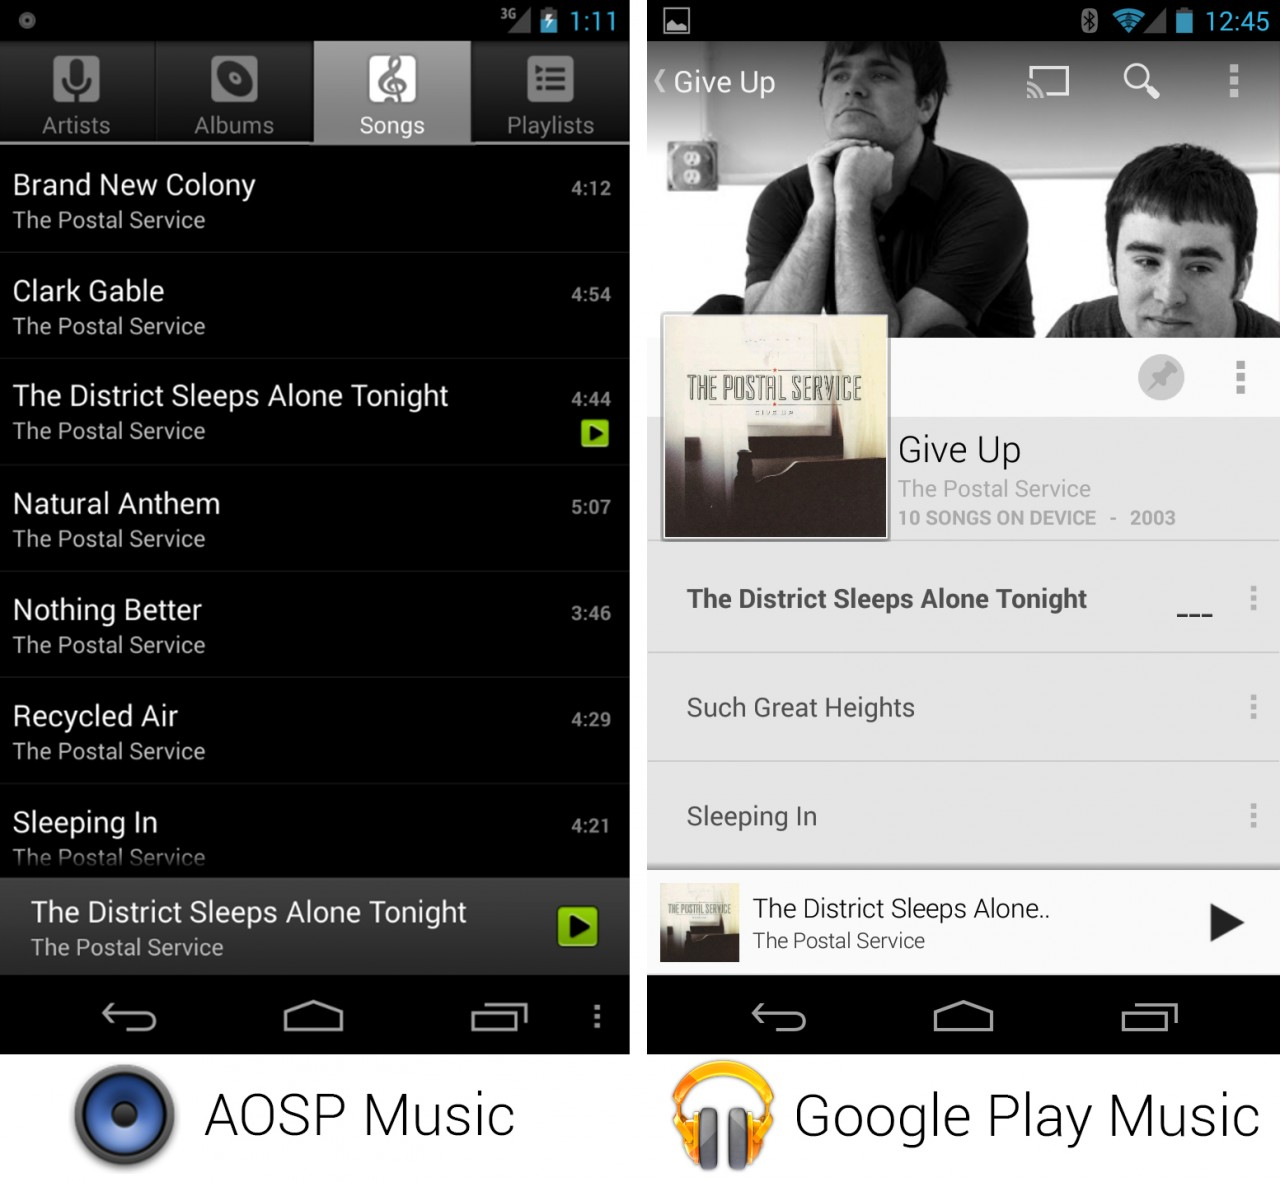
\includegraphics[width=0.55\textwidth]{img/googleplaymusic.jpg}
    \caption{AOSP muziekapplicatie vergeleken met Google's muziekapplicatie}
    \label{fig:googleplaymusic}
    \autocite{amadeo_open-source}
\end{figure}

\begin{figure}
    \centering
    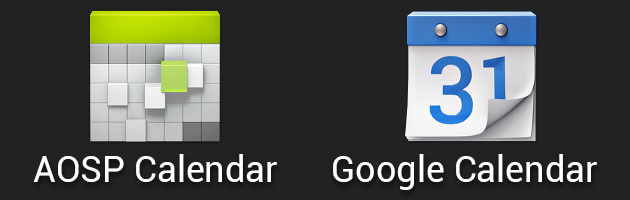
\includegraphics[width=0.55\textwidth]{img/googlecalendar.jpg}
    \caption{AOSP kalender applicatie vergeleken met Google's kalender applicatie}
    \label{fig:googlecalendar}
    \autocite{amadeo_open-source}
\end{figure}

Doordat zeer veel applicaties dus rechtstreeks afhangen van de Google Play Services, zullen veel applicaties ook regelrecht niet meer zoals gewenst functioneren wanneer de Play Services niet aanwezig zijn of deze niet beschikt over de nodige toestemmingen \autocite{marshall_google-play-services}. Android handhaaft een toestemmingssysteem waarbij elke applicatie eerst toestemming moet vragen voordat deze aan gevoelige gebruikersdata kan. Voorbeelden van dergelijke machtigingen zijn toegang tot de camera, contacten en SMS informatie \autocite{android_permissions}. Standaard krijgt Google Play Services, als enige applicatie, alle machtigingen toegekend, zoals te zien in figuur \ref{fig:permissions1}. Wanneer er geprobeerd word om hier de machtigingen in te perken, wordt er ook gemeld dat dit kan leiden tot het verstoren van basisfunctionaliteiten, zoals te zien in figuur \ref{fig:permissions2}. \textquote{Als je deze machtiging weigert, kan het zijn dat basisfuncties van je apparaat niet meer werken zoals bedoeld.}.

\begin{figure}
    \centering
    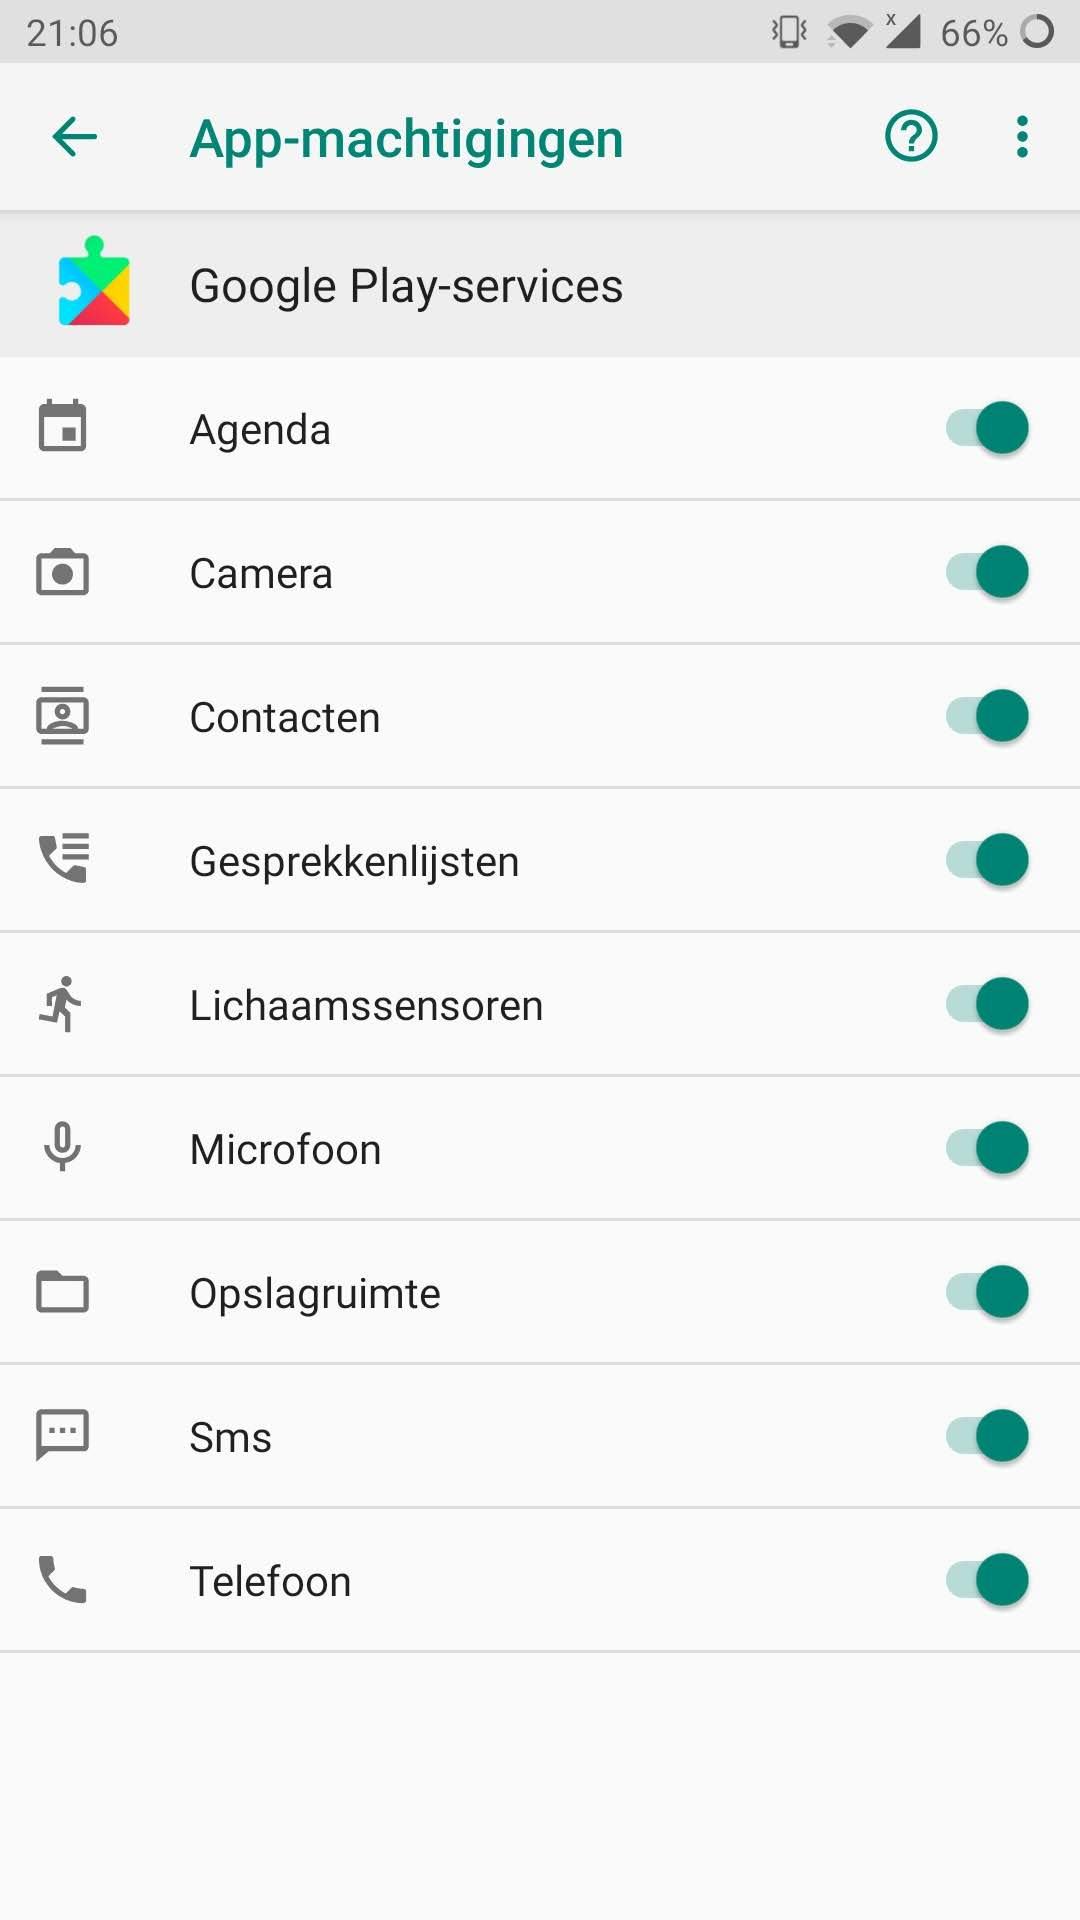
\includegraphics[width=0.4\textwidth]{img/machtigingen.jpg}
    \caption{Screenshot van vereiste machtigingen van Google Play Services}
    \label{fig:permissions1}
\end{figure}

\begin{figure}
    \centering
    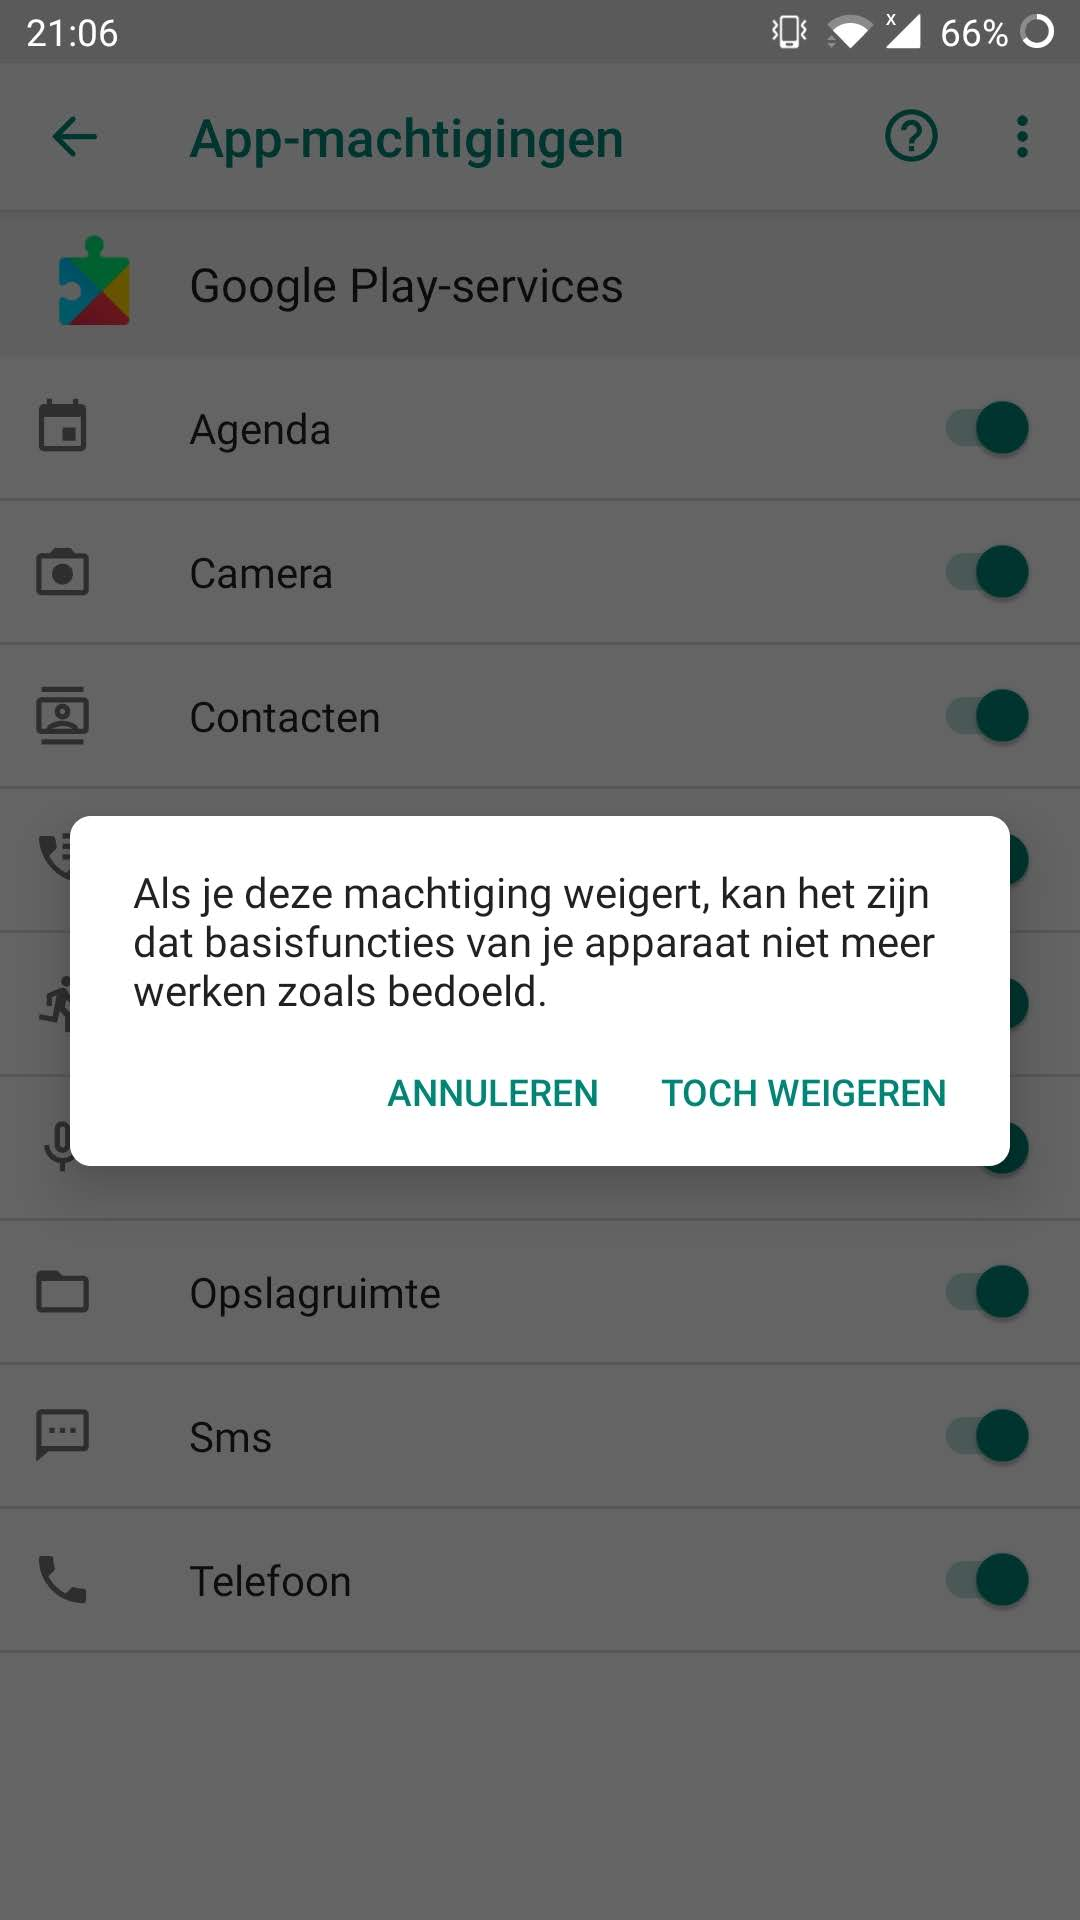
\includegraphics[width=0.4\linewidth]{img/machtigingen_melding.jpg}
    \caption{Screenshot van melding bij inperken van machtigingen van Google Play Services}
    \label{fig:permissions2}
\end{figure}

\subsection{Google Applicaties}

Een ander Google component binnen Android zijn alle Google applicaties. Afhankelijk van de fabrikant van de smartphone, zal er een heel pakket aan Google applicaties samen met de Google Play Services, al dan niet geïnstalleerd zijn. Google applicaties zijn als systeem-applicaties geïnstalleerd, wat betekent dat ze zonder software aanpassingen niet van  het apparaat kunnen verwijderd worden. Wel is het mogelijk om deze applicaties 'uit te schakelen'. Dit houdt in dat ze niet meer op de achtergrond kunnen worden uitgevoerd, en dus ook geen meldingen kunnen sturen.

Applicaties die hier binnenvallen zijn GMail, Google, Google Play Films, Google Play Store, etc.

\section{Door Google verzamelde data}
\label{collected_data}

Deze sectie zal meer informatie geven over de data die door het Android besturingssysteem wordt verzameld. Dit sluit dan ook direct aan op de probleemstelling van deze bachelorproef. Op 15 augustus 2018 publiceerde \textcite{schmidt_google-data-collection}, professor informatica aan Vanderbilt University, een rapport dat in detail het verzamelen van data binnenin het Android besturingssysteem beschrijft. Deze studie van 55 pagina's richtte zich vooral op de oorsprongen en toepassingen van het verzamelen van data die Google gebruikt om zo gebruikersdata te verkrijgen uit beide Google applicaties en hun mobiele besturingssysteem, Android. De informatie binnen deze sectie (\ref{collected_data}) werd verkregen uit dit rapport.

\subsection{Manieren van data-verzameling} \label{ways-of-data-collection}

Google gebruikt verschillende manieren om data te verzamelen. De meest vanzelfsprekende methoden zijn 'actieve', waarbij de gebruiker rechtstreeks en bewust informatie naar Google communiceert. Hieronder valt bijvoorbeeld de situatie waarbij een gebruiker inlogt op een door Google ontwikkelde applicatie, zoals YouTube, gmail, etc. Minder voor de hand liggende manieren die Google gebruikt om data te verzamelen, zijn 'passieve' methoden, waarbij een applicatie geïnstrumenteerd is om data te verkrijgen terwijl deze wordt uitgevoerd, mogelijk zonder dat de gebruiker zich daarvan bewust is. Deze passieve methoden komen voort uit platforms (e.g. Android en Google Chrome), applicaties (e.g. Google Search, Youtube, Google Maps), hulpmiddelen voor uitgevers (e.g. Google Analyticse en AdSense) en hulpmiddelen voor adverteerders (e.g. AdMob en Adwords). Een overzicht van data die verzameld werd op passieve en actieve methoden gedurende één dag is te zien in tabel \ref{tab:collected_data}.

\begin{table}
    \centering
    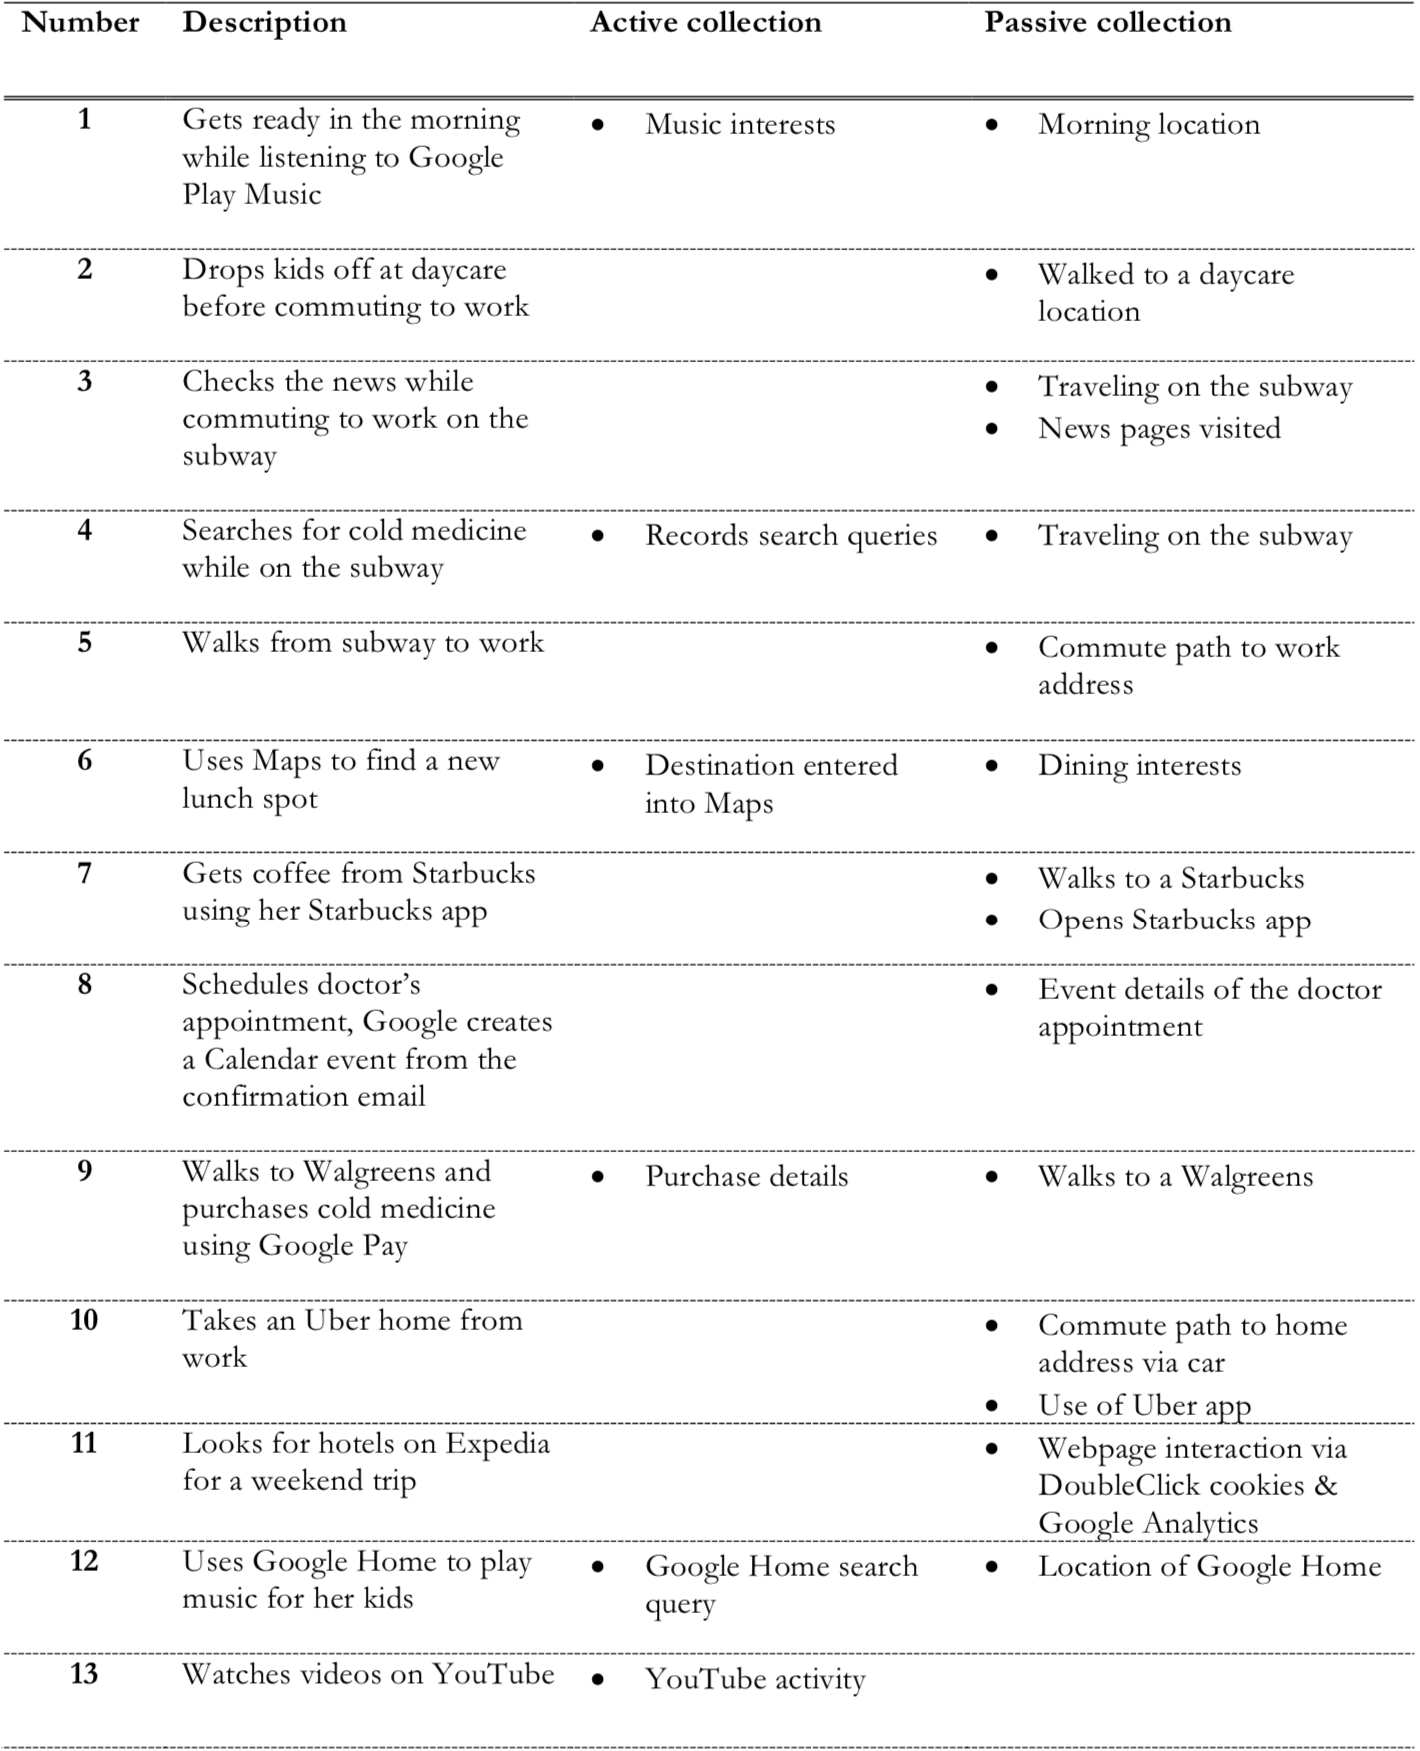
\includegraphics[width=1\textwidth]{img/collecteddata.png}
    \caption{Door Google verzamelde data gedurende één dag}
    \label{tab:collected_data}
    \cite{schmidt_google-data-collection}
\end{table}

\subsection{Bevindingen onderzoek}

Bij typisch internet gebruik van een Android gebruiker, gedurende één dag, kan Google reeds een grote hoeveelheid informatie te weten komen over de persoonlijke interesses van deze gebruiker. In een voorbeeldscenario waarbij een echte gebruiker met een nieuw Google account gebruik maakt van een Android telefoon voor haar dagelijkse routine, bleek dat op verschillende tijdstippen data werd verzameld zoals locatie van de gebruiker, genomen routes, aangekochte items en beluisterde muziek. Twee derden van de verzamelde data, werd verzameld door middel van passieve methoden, zonder dat de gebruiker hiervan op de hoogte werd gebracht. Op het einde van de dag kon Google de interesses van de gebruiker vaststellen met een opmerkelijke precisie.

Het Android besturingssysteem is een essentiële factor bij Google's data-verzameling, aangezien Android meer dan 2 miljard maandelijkse actieve gebruikers heeft. Android helpt Google om persoonlijke gebruikersinformatie (e.g. naam, telefoonnummer, geboortedatum, postcode, en vaak het nummer van de gebruikte kredietkaart), gebruikersactiviteit (e.g. gebruikte applicaties, bezochte websites) en locatiegegevens te verzamelen. Android verstuurt op de achtergrond frequent gegevens naar Google betreffende de locatie van de gebruiker en apparaat gerelateerde informatie zoals applicatie gebruik, crash rapporten, apparaatconfiguratie, backups en andere apparaatgerelateerde identificatiemiddelen.

De Google Chrome internet browser helpt google om gebruikersdata te verzamelen van zowel mobiele apparaten en desktop computers, met meer dan 2 miljard actieve installaties wereldwijd. Deze informatie wordt verzameld wanneer er bv. een online form wordt ingevuld, en dan doorgestuurd naar Google als deel van het data synchronisatie proces. Ook bezochte webpagina's en locatiegegevens worden naar Google toegestuurd.

Zowel Android zelf als Google Chrome sturen data naar Google toe, zonder dat er gebruikersinteractie plaatsvindt. Het uitgevoerde experiment toonde aan dat een Android telefoon die niet bewogen, noch gebruikt werd, 340 keer locatiegegevens doorstuurde naar Google gedurende een periode van 24 uur, met een gemiddelde van 14 communicaties per uur. Deze doorgestuurde locatiegegevens nemen 35\% in van alle uitgestuurde steekproefdata.

Wanneer een gebruiker in contact trad met een Android telefoon (e.g. navigeren door het besturingssysteem, webpagina's bezoeken, apps gebruiken), verhoogde het aantal passieve communicaties naar Google toe significant. Dit gebeurde ook in gevallen waar de gebruiker geen prominente Google applicaties zoals YouTube, Gmail, of Google Maps gebruikte. Deze stijging kan voornamelijk toegewezen worden door data activiteiten van Google's advertentie- en uitgeversproducten, zoals Google Analytics, DoubleClick en AdWords. Deze data maakte 46\% uit van alle uitgaande verzoeken naar Google servers. Google verzamelde 1,4 keer sneller data, wanneer dit vergeleken wordt met het experiment waarbij de Android telefoon volledig stil ligt, zonder gebruikersinteractie. Op vlak van hoeveelheid, communiceerden Google's servers 11.6 MB data met het Android apparaat, per dag. Uit dit experiment kan worden afgeleid dat, zelfs zonder interactie met Google applicaties, Google nog steeds een aanzienlijke hoeveelheid data kan verzamelen door middel van haar advertentie- en uitgeversproducten.

Advertentie-ID's, die vermeend anoniem zijn (ze hangen niet vast aan specifieke gebruikers), verzamelen  gebruikers' activiteiten data bij het gebruik van applicaties en het bezoeken van webpaginas van een derde partij. Deze ID's kunnen gelinkt worden aan de Google identiteit van een gebruiker, doordat identificatiegegevens op apparaatsniveau worden doorgegeven aan Google servers door een Android apparaat. Eveneens wordt ook het DoubleClick cookie ID beschouwd als een anoniem gegeven dat niet vasthangt aan gebruikers. Dit ID volgt gebruikers' activiteiten op webpagina's van een derde partij. Ook deze kunnen worden gelinkt aan een Google account wanneer deze gebruiker een Google applicatie gebruikt in dezelfde browser als degene waarin de webpagina van een derde partij werd bezocht. In het algemeen tonen de bevindingen aan dat Google de mogelijkheid heeft om anoniem verzamelde data te verbinden met de persoonlijke informatie van een gebruiker door middel van passieve methoden.

\section{Mogelijke ontgoogle methoden}

Het doel van het ontgooglen is dan om de Google software zodanig te vermijden zodat je op  een zo min mogelijke manier nog vastzit aan Google. Dit kan op enkele manieren gebeuren, die zullen worden besproken in volgende subsecties.

\subsection{Zachte ingrepen}
\label{softmethods}

Onder zachte ingrepen verstaan we de methoden die enkel gebruik maken van opties die ons rechtstreeks door Android of Google worden aangeboden, zonder softwarematige wijzigingen aan te brengen aan het besturingssysteem.

\subsubsection{Verwijderen van Google account op het apparaat}

Gebruik van een Google account wordt aangeraden bij het gebruik van een Android telefoon, maar is niet verplicht. Bij het instellen van het Android besturingssysteem kunt u de stap om in te loggen bij Google gewoon overslaan. Het is ook mogelijk om een ingelogde Google account later te verwijderen. Enkele applicaties zullen niet werken of gelimiteerde functionaliteit hebben hierdoor, maar mogelijk wil de gebruiker deze Google applicaties niet gebruiken als deze als doel 'ontgooglen' heeft.

\subsubsection{Niet gebruiken van Google applicaties}
Door Google applicaties regelrecht niet te gebruiken, is de grip van Google op Android telefoons al direct een heel stuk zwakker.
Zoals eerder al gezegd, is het niet mogelijk om Google applicaties te verwijderen aangezien ze geïnstalleerd zijn als systeem-applicaties. Ze kunnen echter wel uitgeschakeld worden. Door Google applicaties niet te gebruiken missen we wel redelijk wat basisfunctionaliteiten. De applicaties die dan worden misgelopen, zijn onder andere Google Maps (online kaartendienst), GMail (mail client), Google Foto's (applicatie om foto's bij te houden en te synchroniseren met de cloud), Chrome (internetbrowser), YouTube (online videoplatform), Google Calendar (agenda applicatie), Google Keyboard (toetsenbord), Google Play Store (app-store), etc.  Gelukkig biedt het internet meer dan genoeg alternatieven voor elke Google applicatie. Deze methode zorgt er niet voor dat Google van het besturingssysteem verbannen wordt en het apparaat zal nog steeds communiceren met Google, in de vorm van 'passieve' methoden, zoals besproken in \ref{ways-of-data-collection}. Data die dan nog steeds naar Google kan worden gecommuniceerd zijn bijvoorbeeld locatiegegevens van een gebruiker.

\subsubsection{Uitschakelen van persoonlijke advertenties}
Een mogelijkheid die Google ons geeft, is het uitschakelen van persoonlijke advertenties. Door gebruik te maken van een 'advertising ID' kan Google externen toegang geven tot gebruikersinformatie zoals locatie en apps die gebruikt worden. Google geeft ons de mogelijkheid om toegang tot deze 'advertising ID' uit te schakelen. Dit kan een gebruiker doen door eerst naar het instellingen menu te navigeren, 'Google' te selecteren, en vervolgens 'Advertenties' te selecteren. Hier kan je je door middel van een schuifbalkje afmelden voor personalisatie van advertenties \autocite{knight_degoogle}.

\subsubsection{Uitschakelen van locatie data verzameling}
Standaard stuurt Android heel wat informatie door met betrekking tot de locatie van de gebruiker. Om dit stop te zetten moet een gebruiker binnen zijn google accountinstellingen twee instellingen aanpassen. De eerste hiervan die moet worden uitgeschakeld is 'Locatiegeschiedenis'. Deze functie houdt gedetailleerde gegevens bij over de locaties die een gebruiker bezoekt, om zo gerichte informatie naar deze gebruiker te kunnen sturen. De tweede optie die moet worden uitgeschakeld is 'Web- en app-activiteit'. Wanneer enkel locatiegeschiedenis is uitgeschakeld worden locatiegegevens nog steeds geregistreerd, maar niet meer visueel weergegeven op een persoonlijke tijdlijn. Deze twee instellingen kunnen aangepast worden in de sectie 'Activiteitsopties' binnen de google-accountinstellingen van een gebruiker \autocite{stolzoff_tracking-location-data}. Dit kan op zowel de Android telefoon als via de webpagina gedaan worden, zoals zichtbaar in figuur \ref{fig:activityoptions} en figuur \ref{fig:activityoptions_mobile}.

\begin{figure}
    \centering
    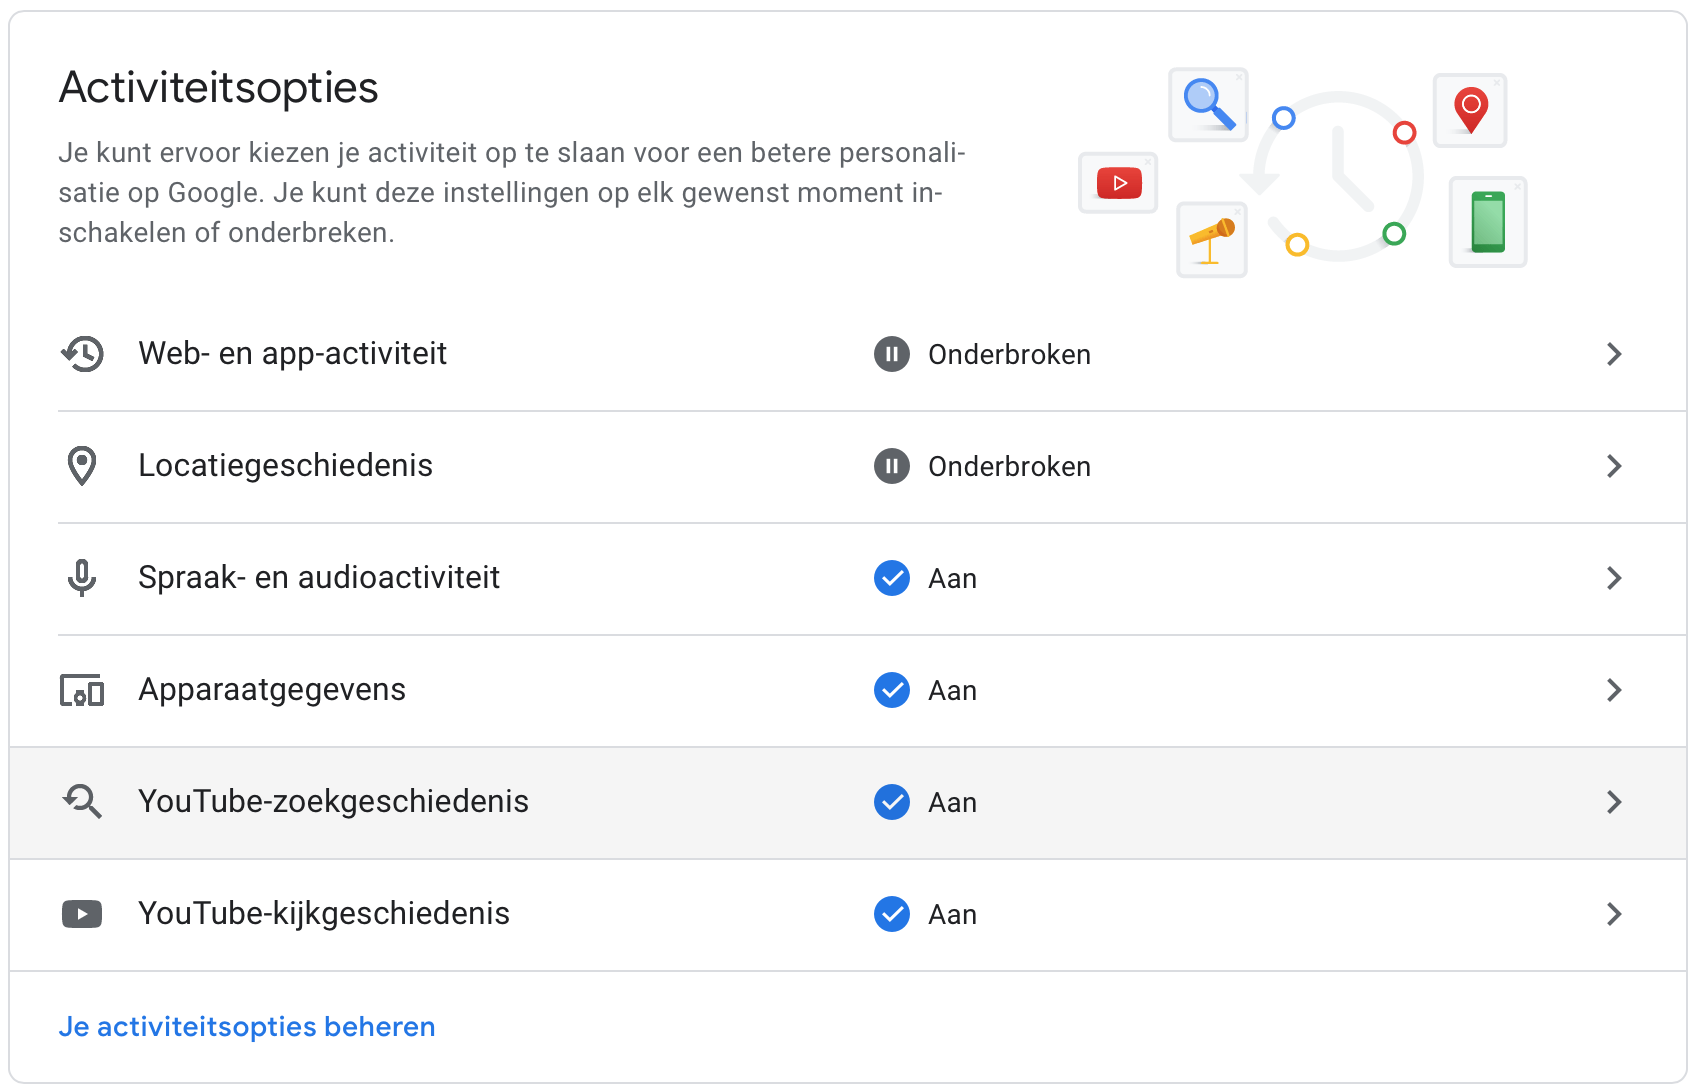
\includegraphics[width=0.8\textwidth]{img/activiteitsopties.png}
    \caption{Screenshot van de instellingen 'Locatiegeschiedenis' en 'Web- en app-activiteit' binnen de web-interface van Google}
    \label{fig:activityoptions}
\end{figure}

\begin{figure}
    \centering
    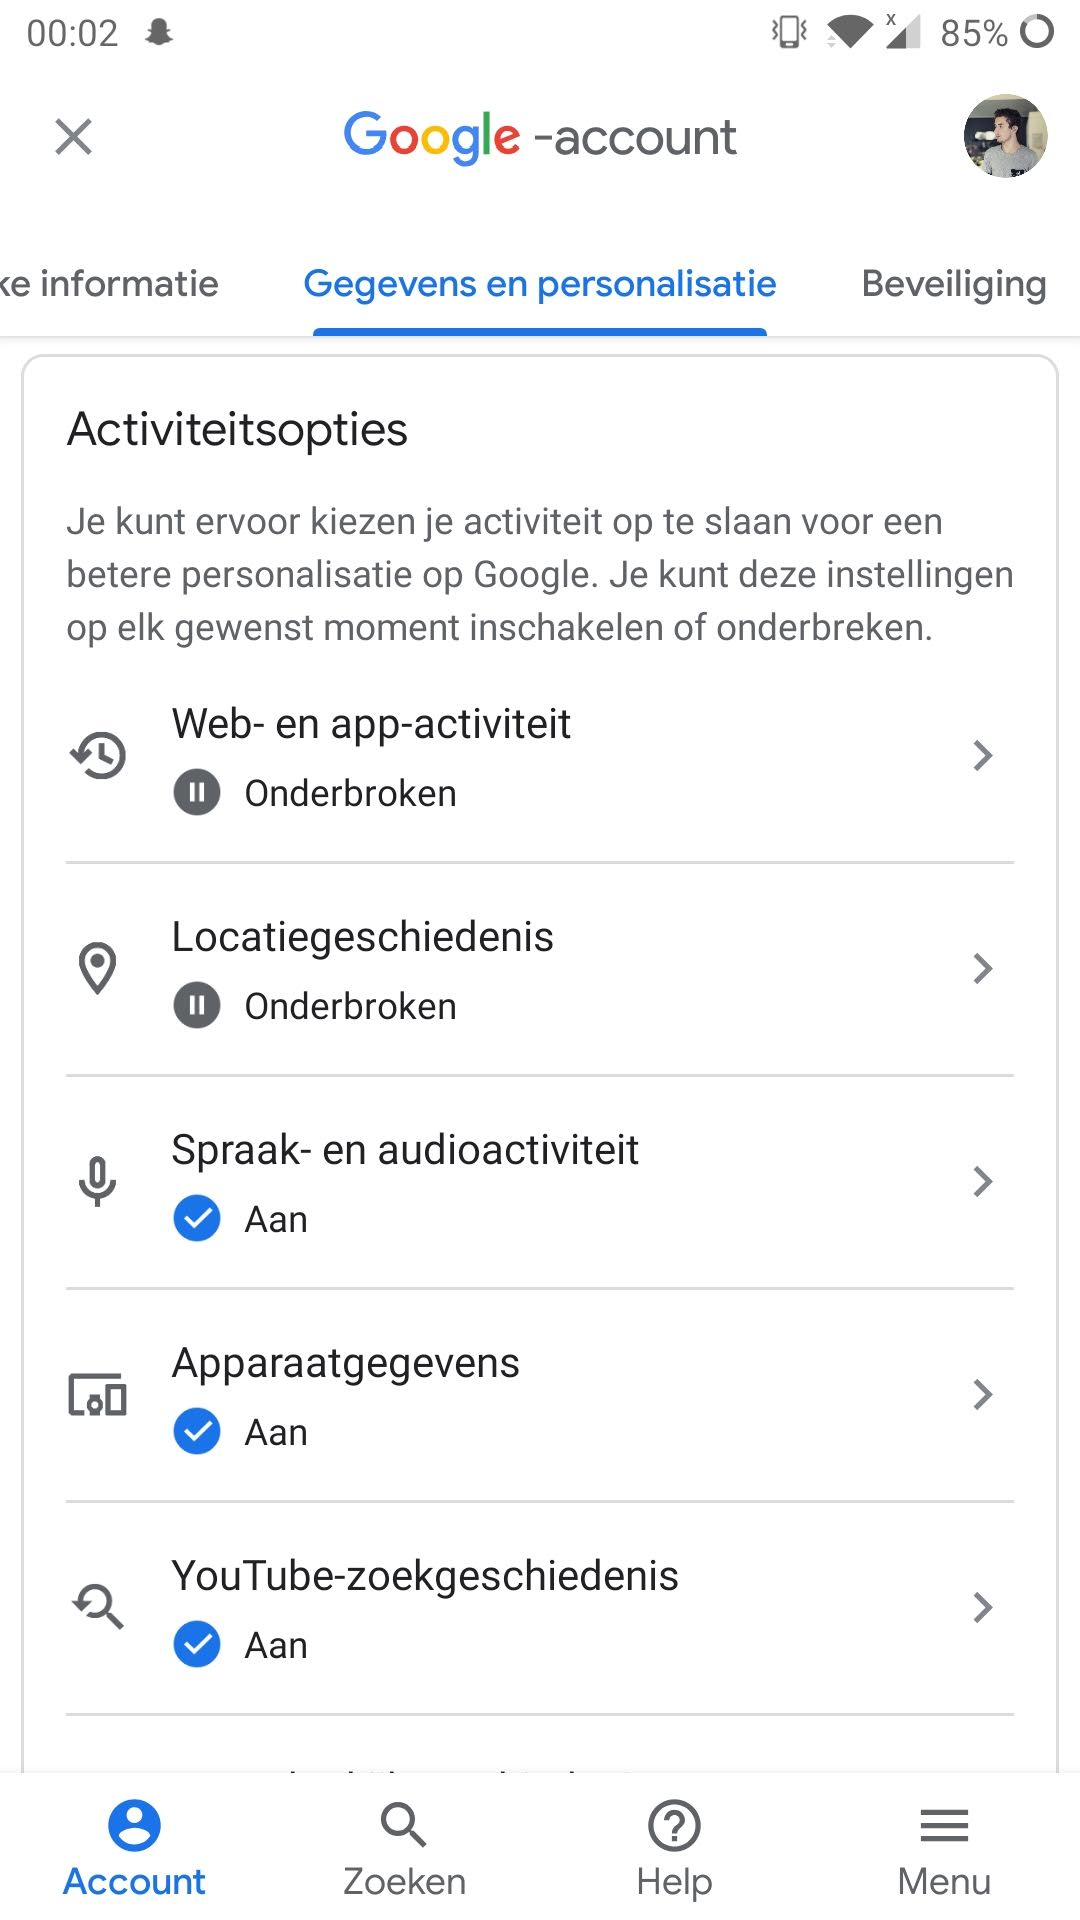
\includegraphics[width=0.4\linewidth]{img/activiteitsopties-mobiel.jpg}
    \caption{Screenshot van de instellingen 'Locatiegeschiedenis' en 'Web- en app-activiteit' in de Google applicatie binnen Android}
    \label{fig:activityoptions_mobile}
\end{figure}


\subsubsection{Veranderen van de standaard DNS server}
Een DNS server is een server, die wanneer je naar een bepaalde site surft, de vertaalstap maakt tussen een domein en het IP adres van de bijhorende webruimte. Als de DNS server van een Android smartphone is ingesteld op de DNS server van Google, kan google het surfgedrag van de gebruiker opvolgen om zo een profiel op te bouwen voor adverteerders. Door de DNS server aan te passen naar één van een andere provider of aanbieder, kan dit worden voorkomen.

Tot Android 8.0, ook wel gekend als Android Oreo, was er geen mogelijkheid om de DNS server bij gebruik van het mobiele netwerk aan te passen, en enkel gelimiteerde mogelijkheden om deze aan te passen bij gebruik van Wi-Fi. Er bestaan echter wel applicaties die door middel van een 'omleiding' en het gebruik van de VPN functie op Android toch hetzelfde resultaat kunnen bekomen \autocite{knight_degoogle}. 

Sinds Android 9.0, ook wel gekend als Android Pie, bestaat DNS-over-TLS. In de instellingen van een Android telefoon kan deze instelling gevonden worden onder 'Wi-FI \& internet' en vervolgens 'Privé-DNS'. Hier kan systeem-wijd een privé-DNS-provider worden ingesteld. Bij het gebruiken van deze functie wordt door middel van encryptie de beveiliging en privacy tussen de client en de DNS-server verbeterd. \autocite{google_dns-tls}

\subsection{Harde ingrepen}

Onder harde ingrepen verstaan we de methoden die gebruik maken van software aanpassingen om zo Google zo veel mogelijk te verbannen.

\subsubsection{Installeren van een Custom ROM}
\label{installcustomrom}
Een 'Android ROM' verwijst naar de versie van AOSP waarop een bepaalde smartphone draait. \autocite{custom-rom}. De versie van Android die vooraf geïnstalleerd is op een smartphone wordt de 'stock ROM' genoemd. Wanneer de gebruiker zijn stock ROM vervangt door een Android ROM die ontwikkeld werd door een externe ontwikkelaar, wordt daarnaar verwezen als een 'custom ROM'. De meeste stock ROM's bevatten standaard reeds de Google Play Services en bijhorende Google applicaties, maar dit is zeker geen vereiste voor het android besturingssysteem. In China is het gebruik van Google verboden, en bijgevolg bevatten toestellen die bedoeld zijn voor de Chinese markt geen enkele verwijzing naar Google software. Doordat de Google Play Store niet kan werken zonder de Google Play Services, moeten chinese bedrijven een eigen 'app store' implementeren om deze te vervangen. Hetzelfde is waar voor custom ROM's. De ontwikkelaar kan zelf kiezen of hij/zij google software wil meeleveren in zijn versie van het besturingssysteem.

Om een custom ROM te installeren, zijn er wel enkele vereisten waaraan een apparaat moet voldoen. Ten eerste moet het apparaat beschikken over een 'unlocked bootloader'. Standaard wordt een Android apparaat geleverd met een 'locked bootloader'. Het hangt dan af van de fabrikant hoe het al dan niet mogelijk is om deze bootloader te unlocken. Het proces om dit te doen verschilt van fabrikant tot fabrikant, en bij meeste fabrikanten houdt dit proces ook in dat alle data op het apparaat wordt gewist. De tweede vereiste om een custom ROM te kunnen installeren is dat er 'custom recovery' geïnstalleerd is. Dit is een gelimiteerde opstartmodus die ons toelaat om de 'custom ROM' te installeren \autocite{hoffman_custom-recovery}.

Als er binnen de custom ROM geen Google software te vinden is, kan een Android telefoon die deze versie van het besturingssysteem draait als 'ontgoogled' beschouwd worden. Dit betekent echter niet dat alle functionaliteiten die voordien werkten, nog steeds allemaal zullen werken. Wanneer applicatie-ontwikkelaars kiezen om tijdens de ontwikkeling verder te werken met een API die wordt aangeboden door de Google Play Services, en niet op een API van AOSP, dan zal deze applicatie hoogstwaarschijnlijk niet werken naar behoren, of zelfs direct crashen wanneer deze geopend wordt.

LineageOS, één van de bekendere custom ROM's, wordt volledig zonder Google Apps geleverd. Dit doen ze omdat licentiebeperkingen dit niet toelaten \autocite{lineage_google-apps}. Het is voor ontwikkelaars van deze custom ROM meestal ook niet interessant om Google Apps op te nemen, aangezien deze zeer vaak worden bijgewerkt. Ze zouden dan bij elke Google App update ook hun ROM moeten bijwerken. Ook is het doelpubliek van custom ROM's vaak op zoek naar een open-source, AOSP ervaring van Android. Daardoor worden Google Apps vaak regelrecht weggelaten \autocite{cawley_gapps}. Hierna is wel nog steeds mogelijk om Google Apps, of een andere implementatie hiervan, apart te installeren. De meest bekende optie om de meeste recente versie van Google Apps te installeren, is 'Open GApps'. Op hun site wordt deze als volgt beschreven: \blockcquote{opengapps_about}{
    The Open GApps Project is an open-source effort to script the automatic generation of up-to-date Google Apps packages.
    On OpenGApps.org you can find more information about the project effort and also pre-built Google Apps packages generated by the OpenGApps.org buildbot.
}
Ook wordt er op hun site gemeld dat zij niet verantwoordelijk zijn voor het verkrijgen van de juiste licensie om deze bestanden te gebruiken.
\blockcquote{opengapps_about}{
    Take note that Open GApps does not provide you with any license for Google’s APKs included in the package. The Open GApps packages merely provide a convenient way to sideload APKs to your device. It is your own responsibility to obtain the proper permissions by e.g. buying an OHA-licensed device with pre-installed Google Apps and/or acquiring the applications from Google’s Play Store.
}

Er bestaat ook een open-source implementatie van de Google Play Services, genaamd microG. Wanneer deze geïnstalleerd wordt bovenop een Google-loze custom ROM, zou het grootste deel van de verloren functionaliteiten hersteld worden. De motivatie voor dit project staat zeer duidelijk uitgelegd op hun site, en luidt als volgt. \blockcquote{microg}{
    The linux-based open-source mobile operating system Android is not only the most popular mobile operating system in the world, it’s also on the way to becoming a proprietary operating system. How is that?
    
    While the core operating system is still released as part of the Android Open Source Project, the majority of core apps are not. It gets worse: More and more libraries and APIs are only available on phones that run various Google apps pre-installed, effectively locking third-party apps to the Google ecosystem. For these reasons Android is described as being a “look but don’t touch” kind of open.
    
    At this point, several popular open-source applications already require some of Google’s proprietary libraries to be installed. Increasing demand in the free software community in addition to severe problems in Google’s proprietary software discovered by the Android modding community, have led to the development of a free software clone of Google’s proprietary core libraries and applications - the microG Project was born.
    
    Although most microG components are far from complete, users are amazed by the results. Free software users got extended application support, privacy-caring users can reduce or monitor data that is sent to Google and especially older phones can expect some battery life improvements. microG is not only used on real devices, but also replaces Google tools in test emulators and is even used in virtual mobile infrastructure.
}
Zoals hierboven vermeld, probeert microG een vervanging te zijn voor de gesloten software van Google, de Google Play Services. Ook wordt er gezegd dat de implementatie van de microG componenten verre van compleet zijn. Het feit dat microG de functionaliteit van de Google Play Services wil nabootsen, impliceert ook dat de nieuwste functies niet direct beschikbaar zullen zijn binnen dit alternatief. Naarmate de ontwikkelaar-gemeenschap achter dit project blijft groeien zal deze functionele achterstand wel inkrimpen.

MicroG maakt het mogelijk om terug de Google Play Store te gebruiken, maar biedt ook een aparte applicatie aan genaamd 'FakeStore'. Deze zorgt ervoor dat andere applicaties denken dat de Play Store aanwezig is, terwijl dit natuurlijk niet zo is. Verder biedt deze applicatie niets van functionaliteit. Alternatieve app-stores zoals F-Droid, de Yalp Store of de Amazon Appstore zijn ook mogelijke opties \autocite{shadow53_play-store}. De Amazon Appstore wordt standaard meegeleverd met apparaten die FireOS als besturingssysteem gebruiken. Amazon probeert zo om Google volledig te vermijden op hun platform, samen met een pakket van nog meer alternatieve services die een vervanging bieden voor die van Google.

\paragraph{SafetyNet}

Aan bovenstaande methode zijn er ook negatieve kanten. Android heeft namelijk veiligheidsmaatregelen getroffen met betrekking tot het blokkeren van veiligheidsrisico's, 'sjoemelen' met het apparaat, kwaadaardige applicaties en 'nep' gebruikers \autocite{android_safetynet}. Dit systeem heet SafetyNet, en maakt deel uit van de Google Play Services. App-ontwikkelaars kunnen via de SafetyNet Attestation API nagaan op welk niveau aan de systeem integriteits controle voldaan wordt. Op basis van deze informatie kunnen bepaalde functies binnen de applicatie geblokkeerd worden. Het is ook mogelijk dat de volledige applicatie onbruikbaar wordt. Denk hier bijvoorbeeld aan het bekende spel 'Pokemon GO', dat het spel onspeelbaar maakt op apparaten die niet aan de SafetyNet controle voldoen. In de Belfius mobiele bankier-applicatie is het bijvoorbeeld niet mogelijk om vingerafdruk-authenticatie te gebruiken op zo'n apparaten. Ook de Play Store kan op basis van deze data het installeren van specifieke applicaties volledig voorkomen.

Wanneer er een custom ROM geïnstalleerd is, is de bootloader ook ontgrendeld (dit is een voorwaarde voor het installeren van een custom ROM). Aan de hand van de CTS (Compatibility Test Suite) kan Google bekijken of er ook maar enige aanpassingen zijn toegepast op het systeem. Een unlocked bootloader valt hier ook onder, en zorgt ervoor dat SafetyNet checks zullen falen.

\paragraph{SafetyNet omzeilen}
Om toch gebruik te kunnen maken van applicaties die het slagen van SafetyNet als vereiste hebben om goed te kunnen functioneren, bestaan er ook oplossingen. Één hiervan heet Magisk. Origineel is Magisk een methode om 'root access' te verschaffen, zonder symsteempartities aan te passen \autocite{topjohnwu_magisk}. Hiernaast biedt Magisk ook methoden om modificaties voor bijna alle systeem-integriteit controle's te verbergen. Dit kan ook gelezen worden op de GitHub pagina van dit project.
\blockcquote{topjohnwu_magiskgithub}{
 Magisk is a suite of open source tools for customizing Android, supporting devices higher than Android 4.2 (API 17). It covers the fundamental parts for Android customization: root, boot scripts, SELinux patches, AVB2.0 / dm-verity / forceencrypt removals etc.
 
 Furthermore, Magisk provides a Systemless Interface to alter the system (or vendor) arbitrarily while the actual partitions stay completely intact. With its systemless nature along with several other hacks, Magisk can hide modifications from nearly any system integrity verifications used in banking apps, corporation monitoring apps, game cheat detections, and most importantly Google's SafetyNet API.
}

Het verkrijgen van root toegang geeft de gebruiker zeer veel macht over het apparaat. Enkele voorbeelden van zaken die mogelijk zijn door het rooten van een Android apparaat, zijn het zien van alle bestanden in het bestandssysteem, een volledige backup nemen van alle applicaties, systeemapplicaties verwijderen, een systeemwijde adblocker, etc. De mogelijkheden zijn haast onbeperkt. Het rooten van een Android apparaat heeft ook nadelen. Een geroot Android apparaat schaadt meestal direct de garantie (afhankelijk van de fabrikant). Het proces, wanneer niet goed uitgevoerd, kan ook zorgen dat het apparaat in een 'gebrickte' staat terechtkomt. In deze staat is het apparaat volledig onbruikbaar. Om uit deze staat te raken is in de meeste gevallen een reeks specifieke stappen nodig, afhankelijk van het specifieke probleem. Wanneer root toegang dan succesvol is verschaft, is het ook zeer makkelijk om een kwaadaardige app volledige toegang te geven over dit apparaat of een instelling fout aan te passen. Deze kunnen dan ook leiden tot een onbruikbaar apparaat \autocite{phelps_root-cons}. Hoewel het Magisk project volledig open-source is, krijgt nog steeds een externe ontwikkelaar de macht over het Android apparaat waarop deze is geïnstalleerd om root toegang te verkrijgen.

\section{Toepassing van Huawei handelsverbod in de Verenigde Staten}
Op 15 mei 2019 voerde president Donald Trump een uitvoeringsbevel door dat ervoor zorgt dat Huawei géén handel meer mag voeren met bedrijven uit de Verenigde Staten. De oorzaak hiervan is minder van belang voor deze bachelorproef, maar de gevolgen sluiten wel dicht aan bij wat er in deze bachelorproef wordt besproken.

Het gebruik van AOSP is gratis en vereist geen contract met Google. Voor het gebruik van Android samen met het 'Google Apps' pakket daarentegen, is een licentie vereist voor apparaten die naar Europa worden verstuurd. Als dit handelsverbod na 90 dagen in werking treedt, zal ook Google verplicht worden deze licentie van Huawei in te trekken. Voor Huawei betekent dit dan concreet dat ze geen software van Google meer mogen meeleveren bij haar besturingssysteem. De afwezigheid van Google is binnen de westerse markt dan ook een zogezegde 'dealbreaker', aangezien dit niet enkel een impact heeft op het gebruik van Google Applicaties (Gmail, Calendar, YouTube, Maps, etc.), maar ook op applicaties die het onderliggende Play Services framework gebruiken. Ook de Play-store zal ontbreken, wat de toegang tot miljoenen applicaties wegneemt. Het is mogelijk voor Huawei om een eigen app-store te ontwikkelen, maar of het hun dan ook lukt om applicaties aan te bieden die de Play-store ook aanbiedt, is een andere vraag.

Andere smartphone producenten zullen uiteraad wel nog Google Apps kunnen blijven leveren binnen hun besturingssystemen, wat hun een groot voordeel geeft over Huawei \autocite{simon_huaweiban}.
